\documentclass[english,twoside, openright, hidelinks, 11 pt, class=report,crop=false]{standalone}
\input{../../preamb}



\begin{document}
{\Large Eksamen Matematikk 10. årstrinn våren 2025\hfill \\ {\footnotesize Løsning fra \color{blue} \href{https://sindreheggen.wordpress.com/}{OpenMathBooks prosjektet}}}	

\subsection*{Oppgave 1}
\textit{Antar her at diagrammet viser antall elevsvar (i motsetning til prosentdeler av elevsvar)} \os

Ser at det totalt er 100 elevsvar. Det betyr at vi kan behandle tallene både som et antall og som et prosenttall.

\begin{center}
	\begin{tabular}{l | l | l}
		\textbf{Påstand} & \textbf{Sann/usann} & \textbf{Forklaring} \\ \hline
		Nesten $\frac{2}{3}$ av elevene spiser lunsj på skolen& Sann & $\frac{2}{3}\approx67\%\approx65\%$ \\ \hline
		Det er litt mer enn tre ganger & &\\ så mange elever som spiser lunsj på 
		skolen & & \\ 5 dager i uka, enn de som spiser grønnsaker,& &\\ frukt og bær på
		skolen 5 dager i uka & Sann & $65>3\cdot21=63$ \\ \hline
		60\% av ungdommene spiser grønnsaker, & &\\ 
		frukt eller bær 3 dager eller
		mer i uka. & Usann &  $\frac{21+17}{100}<\frac{60}{100}$ \\ \hline
		$\frac{1}{4}$ av elevene spiser & &\\ lunsj på skolen 1-4 dager i uka & Sann & $\frac{17+8}{100}=\frac{1}{4}$ 
	\end{tabular}
\end{center}


\subsection*{Oppgave 2}
\abc{
\item $\frac{11}{20}=\frac{55}{100}$, altså er $55\%$ rett alternativ.
\item 

\textbf{Alternativ 1}\\
Nytt antall skudd er 30. Da $60\%=\frac{3}{5}=\frac{18}{30}$, må nye skåringer være lik $18-11=7$.

\textbf{Alternativ 2}\\
Vi setter antall nye skåringer lik $x$. Da $60\%=\frac{3}{5}$, har vi at
\begin{align}
\frac{11+x}{30}&=\frac{3}{5}	\\
11+x&=18 \\
x&=7
\end{align}
}
\subsection*{Oppgave 3}
Setter $\text{pris for baguett}=y$ o $\text{pris for salat}=x$. Da er
\begin{align}
	30x+40y &= 1600 \label{opg3a} \vn
	22x+40y&=1440 \label{opg3b}
\end{align}
Vi trekker ligning \eqref{opg3b} fra ligning \eqref{opg3a}, og får at
\begin{align*}
	30x+40y-(22x+40y)&=1600-1440\\
	8x &= 160\\
	x&=20
\end{align*}
Vi setter denne verdien for $x$ inn i \eqref{opg3a}:
\begin{align}
	30\cdot20+40y&=1600 \\
	40y &= 1600-600 \\
	40y &= 1000 \\
	y &= 25
\end{align}

\subsection*{Oppgave 4}
Grafen ser ut til å skjære punktene $(0, 6)$ og $(30, 0)$. Stigningstallet er da
\[ \frac{0-6}{30-0}=-\frac{1}{5}=-0.2 \]
\subsection*{Oppgave 5}
\abc{
\item Lengde 40\enh{cm}, bredde 30\enh{cm}, høyde 60\enh{cm}
\item Gjør om benevningen til dm. $3\cdot4\cdot6=72$, altså er volumet 72\enh{L}.
}

\subsection*{Oppgave 5}
\abc{
\item $(2+4)(10-4)=6\cdot6=36$
\item Setter $a=4$ og $b=10$. $(4+2)(10-6)=6\cdot4=24$. \\ 24 kan faktoriseres på flere måter med to faktorer, ${12\cdot2=24}$ og $8\cdot3=24$. Ved å velge rett $a$ og $b$ kan vi få disse faktorene.
}

\subsection*{Oppgave 6}
\abc{
\item I linje 1-3 skriver man inn sidelengdene til trekanten.

I linje 5 sjekker man om sidelengdene oppfyller Pytagoras' setning. Hvis ja, printes "Trekanten er rettvinklet", hvis nei printes "Trekanten er ikke rettvinklet".
\item $5^2+6^2=25+36\neq 8^2=64$, dermed vil programmet svare at "Trekanten er ikke rettvinklet".
}

\newpage
\subsection*{Oppgave 1}
\abc{
\item \phantom{}\\
\begin{tabular}{c c c c c}
	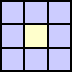
\includegraphics{opg1d1a} & 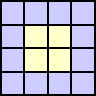
\includegraphics{opg1d1b} & 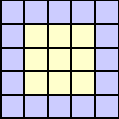
\includegraphics{opg1d1c} & 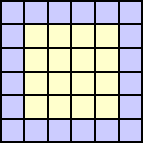
\includegraphics{opg1d1d} & 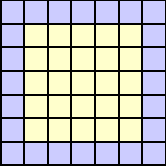
\includegraphics{opg1d1e} \\
	Figur 1 & Figur 2 & Figur 3 & Figur 4 & Figur 5
\end{tabular}
\item \phantom{}
\begin{figure}
	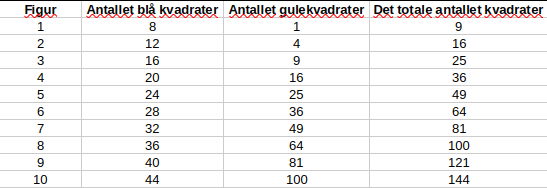
\includegraphics[scale=0.5]{opg1del1db}
\end{figure}
\item 
\begin{align*}
	&\text{Det totale antallet kvadrater}=(n+2)^2 \\
	&\text{Antallet gule kvadrater}= n^2\\
	&\text{Antallet blå kvadrater}=\text{Totalt antall}-\text{Antall gule}=(n+2)^2-n^2=4(n+1)
\end{align*}
For $n=4$ får vi at
\[ \text{Antallet blå kvadrater}=4(4+1)=20 \]
}

\newpage
\subsection*{Oppgave 2}
\textit{Antar at det er ønskelig å gå for tilbudet som gir lavest pris per par.}\os

\textbf{Tilbud 1}\\
$\text{Antall kroner per par}=\frac{299}{6}\approx 50$ \os

\textbf{Tilbud 2} \\
$25\% \text{ av } 80=0.25\cdot80=20$, altså koster det 60\enh{kr} per par. \os

\textbf{Tilbud 3} \\
$\text{Antall kroner per par}=\frac{2\cdot80}{3}\approx 53$\os

\textbf{Tilbud 4}\\
Par nummer tre koster 40\enh{kr}. $\text{Antall kroner per par}=\frac{2\cdot80+40}{3}\approx 67$\vsk

Tilbud 1 gir lavst pris per par.


\subsection*{Oppgave 3}
\abc{
\item 20 000 er beløpet (i kroner) han setter inn i banken. \\
1,04 er vekstfaktoren ved 4\% sparerente.\\
$x$ er antall år etter at beløpet ble satt inn.
\item \[ \text{Penger i banken etter 15 år}=20000\cdot1,04^15\approx 36019 \]
Etter 15 år vil han ha ca. 36\,019\enh{kr} i banken.
}

\subsection*{Oppgave 4}
\abc{
\item På terningen er 1, 3 og 5 oddettall, mens 2, 4, og 6 er partall. Det betyr at det er like mange av hver, og derfor lik sannsynlighet.
\item Antar at Masa ikke legger tilbake ballen hun trekker. Når Masa har trukket en ball, er det 1 ball av totalt 3 baller som har fargen Agata ønsker å trekke. Altså har Agata bare $\frac{1}{3}$ sjanse for å trekke samme farge som Masa.
}

\subsection*{Oppgave 5}
\begin{comment}
	For jentene er variasjonsbredden $6-1=5$, for guttene er den $7-1=6$. Variasjonsbredden er et spredningsmål.\os
\textbf{Alternativ 1 (sentralmål)} \os
\textbf{Jenter}
\[
\footnotesize 1\qquad2\qquad2\qquad2\qquad3\qquad3\qquad3\qquad3\qquad3\qquad4\qquad5\qquad5\qquad5\qquad6 \]
Typetall: 3 \\
Median: $\frac{3+3}{2}=3$ \\
Gjennomsnitt: $ \frac{1+2+2+2+3+3+3+3+3+4+5+5+5+6}{14}\approx 3,36$ \vsk

\textbf{Gutter}
\[ \footnotesize 1\qquad1\qquad1\qquad2\qquad2\qquad2\qquad2\qquad2\qquad3\qquad3\qquad3\qquad4\qquad5\qquad6\qquad7\]
Typetall: 2\\ 
Median: 2 \\
Gjennomsnitt: $\frac{1+1+1+2+2+2+2+2+3+3+3+4+5+6+7}{15}\approx 2,93 $
\end{comment}
\begin{figure}
	\centering
	
\includegraphics[scale=0.3]{opg5a}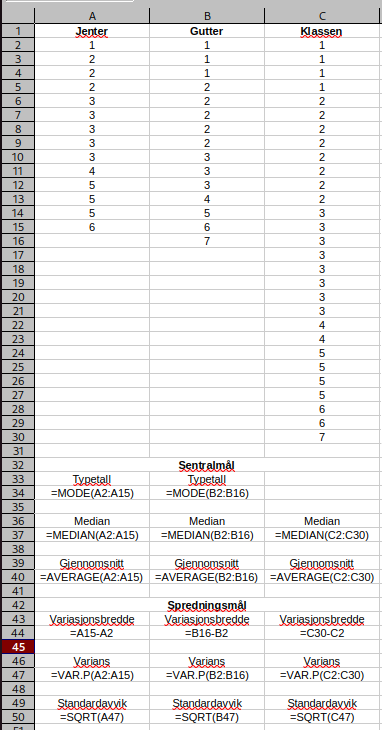
\includegraphics[scale=0.2]{opg5b}
\end{figure}
\begin{itemize}
	\item For både jentene, guttene og klassen samlet er median og gjennomsnitt ganske like i verdi. Dette er å forvente da verdiene har en ganske jevn stigning på hver side av medianen.
	\item Klassen har ikke et typetall siden det både er åtte 2ere og åtte 3ere.
	\item Standardavviket til guttene er litt høyere enn det til jentene. Det samsvarer med at guttene har større variasjonsbredde enn jentene.
	\item Valgte å lage et søylediagram da dette gir en rask sammenligning av jentene og guttene.
\end{itemize}

\newpage
\subsection*{Oppgave 6}
\textit{Antar at elevrådet er ute etter lavest mulig total pris (i motsetning til pris per elev).} \vsk

Vi lar pris per elev være lik $x$, og skriver inn Tilbud 1 og Tilbud 2 som $f$ og $g$ i GeoGebra. Tilbud 3 er representert ved linja $y=7000$, men er bare gyldig frem til $x=70$.
\begin{itemize}
	\item Opp til 40 elever er Tilbud 1 billigst (linje 3).
	\item Mellom 40 og 53 elever er Tilbud 2 billigst (linje 3 og linje 7).
	\item Tilbud 3 vil lønne seg hvis det kommer mellom 53 og 70 elever. Hvis det kommer flere enn 70 elever, er ikke Tilbud 3 gyldig. Da er Tilbud 2 billigst. 
\end{itemize}
\begin{figure}
	
\includegraphics[scale=0.35]{opg6}
\end{figure}
\newpage
\subsection*{Oppgave 7}
\abc{
\item \begin{itemize}
	\item Både deltakelse i organisert idrett og uorganisert idrett går jevnt nedover jo eldre man blir.
	\item Egentrening går først jevnt nedover jo eldre man blir, men tar seg litt opp igjen når man er på VG3. Da er det samme nivå som i 10. klasse. 
	\item Deltakelse på treningsstudio øker hvert år ganske mye mellom 8. til 10. klasse. Deltakelsen øker også på videregående, men der er økningen mindre (0 mellom 1. og 2. VGS).
\end{itemize}
\item Både Mira og Per har brukt tallene fra søylediagrammet med undertittel "Idrettslag", men det er feil av Mira å presentere dette som nedgang i medlemstall over tid. Tallene viser hvordan medlemstallene fordeler seg over de forskjellige årstrinnene. At mange slutter i idrettslag når de blir eldre betyr ikke at idrettslag får færre medlemmer over tid. Per sitt råd er basert på en riktig tolkning av tallene.
}

\newpage
\subsection*{Oppgave 8}
\abc{
\item Påstand 1 stemmer her: $3+5=8$, $7+7=14$ \\
Påstand 2 stemmer ikke her: $1+2=3$, $10+11=21$ \\
Påstand 3 stemmer her: $1+2+3=6$\\
Påstand 3 stemmer ikke her: $2+3+4=9$
\item Påstand 1 vil alltid stemme. Påstand 2 vil aldri stemme. Påstand 3 vil noen ganger stemme.
\item La $n$ og $k$ være heltall. Da er $2n$ og $2k$ partall og $2n+1$ og $2k+1$ oddetall.\os

For Påstand 1 har vi at
\[ \text{Summen av to oddetall}=2n+1+2k+1=2(n+k+1)\]
Da 2 er en faktor i uttrykket, vil $2(n+k+1)$ alltid være et partall. \vsk

For Påstand 2 har vi at
\[ \text{Summen av to påfølgende heltall}=2n+2n+1=4n+1 \]
Da $4n$ er et partall, må $4n+1$ være et oddetall.\vsk

For Påstand 3 har vi at
\begin{itemize}
	\item Hvis det første heltallet er et partall, har vi at
	\[ \text{sum}=2n+2n+1+2n+2=6n+3 \]
	Da $6n$ er et partall, er $6n+3$ et oddetall.
	\item  Hvis det første heltallet er et oddetall, har vi at
	\[ \text{sum}=2n+1+2n+2+2n+3=6n+4=2(2n+2) \]
	Da 2 er en faktor i uttrykket, vil $2(2n+2)$ alltid være et partall.
\end{itemize}



}
\end{document} 